% ================================================================ 18
\section{Pruebas}
\label{sec:pruebas}

Esta sección documenta la batería de pruebas realizadas sobre \ggez\ para verificar su funcionamiento. Las pruebas se organizan según las categorías establecidas por el enunciado del proyecto, y cada una indica su objetivo, entrada, resultado esperado, resultado obtenido y estado (aprobada o reprobada).

Cada caso es un proyecto \ggez\ real guardado en el repositorio, dentro de una carpeta por categoría en \kw{Traductor/pruebas/}: \kw{1\_validos/}, \kw{2\_sintacticos/}, \kw{3\_semanticos/}, \kw{4\_importaciones/}, \kw{5\_circular/}, \kw{6\_completa/} y \kw{7\_advertencias/}. Cada caso tiene su \kw{principal.ggez} (con una cabecera de comentarios que documenta la prueba, su objetivo y su entrada), un archivo \kw{esperado.txt} con la salida esperada completa (salida estándar, salida de errores y código de salida) y, si el programa lee datos, un archivo \kw{entrada.txt}.

El script \kw{pruebas/correr.py} ejecuta cada caso con el traductor real y compara la salida obtenida con la esperada; se ejecuta con \kw{make test} desde la carpeta \kw{Traductor}. Las tablas de esta sección se generaron con ese mismo script (\kw{python pruebas/correr.py --latex}), por lo que el resultado obtenido corresponde a una ejecución real. Los números de línea de los mensajes corresponden al archivo del caso, incluida su cabecera de comentarios. Las 23 pruebas resultaron aprobadas.

\begin{longtable}{|p{7.4cm}|p{2.6cm}|p{2.6cm}|}\hline
\cab\textbf{Categoría} & \textbf{Casos} & \textbf{Aprobados} \\\hline\endhead
Programas válidos & 5 & 5 \\\hline
Errores sintácticos & 5 & 5 \\\hline
Errores semánticos & 5 & 5 \\\hline
Importaciones & 5 & 5 \\\hline
Importación circular & 1 & 1 \\\hline
Prueba completa relacionada con el problema & 1 & 1 \\\hline
Advertencias & 1 & 1 \\\hline
\textbf{Total} & \textbf{23} & \textbf{23} \\\hline
\end{longtable}

\subsection{Programas válidos}
\label{pr:1_validos}
Casos de la carpeta \texttt{pruebas/1\_validos/}.

\begin{tablaprueba}
1. Tipos simples y operaciones. Declarar los cinco tipos simples y una constante, y usar operaciones aritméticas, relacionales y lógicas & \texttt{1\_\allowbreak{}validos/\allowbreak{}01\_\allowbreak{}tipos\_\allowbreak{}y\_\allowbreak{}operaciones}. Entrada: ninguna & {\ttfamily\footnotesize Novato (rango B)\newline Vida tras 2 golpes: 70\newline Dano critico: 11.25\newline 17 split 5 = 3, 17 scrap 5 = 2\newline Sigue vivo: hit\newline Sin escudo: miss\newline Vida igual a 100: hit, distinta de 50: hit\newline [codigo de salida 0]} & Igual al esperado. \textbf{Aprobada} \\ \hline
2. Entrada de datos y condicionales. Leer datos con chat.load y decidir con scan, fallback y loadout & \texttt{1\_\allowbreak{}validos/\allowbreak{}02\_\allowbreak{}entrada\_\allowbreak{}y\_\allowbreak{}condicionales}. Entrada: Ana y mago & {\ttfamily\footnotesize Nombre del jugador:\newline Clase (guerrero, mago o arquero):\newline Bienvenido, Ana. Poder: 95\newline Rango: Pro\newline [codigo de salida 0]} & Igual al esperado. \textbf{Aprobada} \\ \hline
3. Ciclos. Usar farm (for), survive (while) y grind (do-while), con ragequit y respawn & \texttt{1\_\allowbreak{}validos/\allowbreak{}03\_\allowbreak{}ciclos}. Entrada: ninguna & {\ttfamily\footnotesize Monedas (1..6 sin el 3): 18\newline Quedan 3 enemigos\newline Quedan 2 enemigos\newline Quedan 1 enemigos\newline El grind corre al menos una vez\newline [codigo de salida 0]} & Igual al esperado. \textbf{Aprobada} \\ \hline
4. Funciones, recursión y squad. Combos con y sin retorno, parámetros, recursión directa y operaciones de squad & \texttt{1\_\allowbreak{}validos/\allowbreak{}04\_\allowbreak{}funciones\_\allowbreak{}y\_\allowbreak{}listas}. Entrada: ninguna & {\ttfamily\footnotesize 5! = 120\newline - Tanque\newline - Sanador\newline - Arquero\newline Ahora son 2, el primero es Curandero\newline [codigo de salida 0]} & Igual al esperado. \textbf{Aprobada} \\ \hline
5. Registros, clases, herencia y manejo de errores. Usar inventory, guild con evolves y clutch/revive/checkpoint & \texttt{1\_\allowbreak{}validos/\allowbreak{}05\_\allowbreak{}objetos\_\allowbreak{}y\_\allowbreak{}errores}. Entrada: ninguna & {\ttfamily\footnotesize Espada tiene poder 40\newline Conan: POR LA GLORIA!\newline Error atrapado en la linea 44: division entre cero\newline El checkpoint siempre corre\newline [codigo de salida 0]} & Igual al esperado. \textbf{Aprobada} \\ \hline
\end{tablaprueba}

\subsection{Errores sintácticos}
\label{pr:2_sintacticos}
Casos de la carpeta \texttt{pruebas/2\_sintacticos/}.

\begin{tablaprueba}
1. Bloque sin cerrar. Detectar un glhf al que le falta su gg & \texttt{2\_\allowbreak{}sintacticos/\allowbreak{}01\_\allowbreak{}bloque\_\allowbreak{}sin\_\allowbreak{}gg}. Entrada: ninguna & {\ttfamily\footnotesize principal.ggez:5:30: error sintactico: bloque sin cerrar: falta 'gg'\newline     posible causa: Cada glhf necesita su gg. Revise que no se haya borrado un gg al final de un bloque.\newline [codigo de salida 1]} & Igual al esperado. \textbf{Aprobada} \\ \hline
2. Combo sin drops. Detectar un combo que no declara su tipo de retorno con drops & \texttt{2\_\allowbreak{}sintacticos/\allowbreak{}02\_\allowbreak{}combo\_\allowbreak{}sin\_\allowbreak{}drops}. Entrada: ninguna & {\ttfamily\footnotesize principal.ggez:5:25: error sintactico: se esperaba 'drops' y se encontro 'glhf'\newline     posible causa: Revise el orden de las palabras en esta linea comparandolo con la sintaxis en Ayuda.\newline [codigo de salida 1]} & Igual al esperado. \textbf{Aprobada} \\ \hline
3. Punto de entrada mal escrito. Detectar que start THE GAME es texto fijo obligatorio & \texttt{2\_\allowbreak{}sintacticos/\allowbreak{}03\_\allowbreak{}punto\_\allowbreak{}de\_\allowbreak{}entrada\_\allowbreak{}mal\_\allowbreak{}escrito}. Entrada: ninguna & {\ttfamily\footnotesize principal.ggez:5:20: error sintactico: se esperaba 'THE' y se encontro 'GAME'\newline     posible causa: Revise el orden de las palabras en esta linea comparandolo con la sintaxis en Ayuda.\newline [codigo de salida 1]} & Igual al esperado. \textbf{Aprobada} \\ \hline
4. Condicional sin glhf. Detectar un scan cuya condición no va seguida de glhf & \texttt{2\_\allowbreak{}sintacticos/\allowbreak{}04\_\allowbreak{}scan\_\allowbreak{}sin\_\allowbreak{}glhf}. Entrada: ninguna & {\ttfamily\footnotesize principal.ggez:7:21: error sintactico: se esperaba 'glhf' y se encontro un salto de linea\newline     posible causa: Revise el orden de las palabras en esta linea comparandolo con la sintaxis en Ayuda.\newline [codigo de salida 1]} & Igual al esperado. \textbf{Aprobada} \\ \hline
5. Declaración sin valor. Detectar un set al que le falta la expresión & \texttt{2\_\allowbreak{}sintacticos/\allowbreak{}05\_\allowbreak{}falta\_\allowbreak{}valor}. Entrada: ninguna & {\ttfamily\footnotesize principal.ggez:6:25: error sintactico: se esperaba una expresion y se encontro un salto de linea\newline     posible causa: Revise el orden de las palabras en esta linea comparandolo con la sintaxis en Ayuda.\newline [codigo de salida 1]} & Igual al esperado. \textbf{Aprobada} \\ \hline
\end{tablaprueba}

\subsection{Errores semánticos}
\label{pr:3_semanticos}
Casos de la carpeta \texttt{pruebas/3\_semanticos/}.

\begin{tablaprueba}
1. Variable no declarada. Detectar el uso de una variable que nunca se declaró con stash & \texttt{3\_\allowbreak{}semanticos/\allowbreak{}01\_\allowbreak{}no\_\allowbreak{}declarada}. Entrada: ninguna & {\ttfamily\footnotesize principal.ggez:7:25: error semantico: 'escudo' no esta declarada\newline     posible causa: Declarela con stash antes de usarla, o revise si escribio mal el nombre o si quedo en otro bloque.\newline [codigo de salida 1]} & Igual al esperado. \textbf{Aprobada} \\ \hline
2. Tipos incompatibles. Detectar que se guarda un lore en una variable score & \texttt{3\_\allowbreak{}semanticos/\allowbreak{}02\_\allowbreak{}tipos\_\allowbreak{}incompatibles}. Entrada: ninguna & {\ttfamily\footnotesize principal.ggez:6:5: error semantico: se esperaba score y se obtuvo lore\newline     posible causa: Los tipos no coinciden: use un valor del tipo declarado (score, aim, lore, win, pixel...).\newline [codigo de salida 1]} & Igual al esperado. \textbf{Aprobada} \\ \hline
3. Cantidad de argumentos. Detectar una llamada con menos argumentos que parámetros & \texttt{3\_\allowbreak{}semanticos/\allowbreak{}03\_\allowbreak{}cantidad\_\allowbreak{}argumentos}. Entrada: ninguna & {\ttfamily\footnotesize principal.ggez:10:21: error semantico: el combo 'atacar' espera 2 argumento(s) y recibio 1\newline     posible causa: Revise la firma del combo: la cantidad de valores entre \{ \} debe ser igual a la de parametros.\newline [codigo de salida 1]} & Igual al esperado. \textbf{Aprobada} \\ \hline
4. Redeclaración. Detectar dos stash con el mismo nombre en el mismo bloque & \texttt{3\_\allowbreak{}semanticos/\allowbreak{}04\_\allowbreak{}redeclaracion}. Entrada: ninguna & {\ttfamily\footnotesize principal.ggez:7:5: error semantico: 'oro' ya fue declarada en este bloque\newline     posible causa: Para cambiar su valor use set sin stash.\newline [codigo de salida 1]} & Igual al esperado. \textbf{Aprobada} \\ \hline
5. Archivo principal sin punto de entrada. Detectar que el archivo principal no tiene lobby.launch & \texttt{3\_\allowbreak{}semanticos/\allowbreak{}05\_\allowbreak{}sin\_\allowbreak{}punto\_\allowbreak{}de\_\allowbreak{}entrada}. Entrada: ninguna & {\ttfamily\footnotesize principal.ggez:1:1: error semantico: el programa no tiene punto de entrada: falta lobby.launch\{start THE GAME\}\newline     posible causa: Agregue lobby.launch\{start THE GAME\} glhf ... gg en el archivo principal.\newline [codigo de salida 1]} & Igual al esperado. \textbf{Aprobada} \\ \hline
\end{tablaprueba}

\subsection{Pruebas de importaciones}
\label{pr:4_importaciones}
Casos de la carpeta \texttt{pruebas/4\_importaciones/}.

\begin{tablaprueba}
1. Importación válida. Usar combos y tipos de un archivo de la misma carpeta (base) y de una subcarpeta (lib) & \texttt{4\_\allowbreak{}importaciones/\allowbreak{}01\_\allowbreak{}importacion\_\allowbreak{}valida}. Entrada: ninguna & {\ttfamily\footnotesize Dano: 60\newline Pocion cuesta 25 monedas\newline [codigo de salida 0]} & Igual al esperado. \textbf{Aprobada} \\ \hline
2. Archivo importado inexistente. Detectar un travel a un archivo que no existe & \texttt{4\_\allowbreak{}importaciones/\allowbreak{}02\_\allowbreak{}archivo\_\allowbreak{}inexistente}. Entrada: ninguna & {\ttfamily\footnotesize principal.ggez:5:1: error de importacion: no existe inventario.ggez en la misma carpeta\newline     posible causa: Revise el nombre del archivo o tipo y la carpeta indicada en el from.\newline [codigo de salida 1]} & Igual al esperado. \textbf{Aprobada} \\ \hline
3. Combo inexistente en el módulo. Detectar la llamada a un combo que el archivo importado no define & \texttt{4\_\allowbreak{}importaciones/\allowbreak{}03\_\allowbreak{}combo\_\allowbreak{}inexistente}. Entrada: ninguna & {\ttfamily\footnotesize principal.ggez:8:22: error de importacion: el modulo combate no tiene 'curar'. Tiene: danoTotal\newline     posible causa: Revise el nombre: el mensaje lista lo que si existe.\newline [codigo de salida 1]} & Igual al esperado. \textbf{Aprobada} \\ \hline
4. Tipos incompatibles en una llamada importada. Detectar que se pasa un lore a un parámetro score de un combo de otro archivo & \texttt{4\_\allowbreak{}importaciones/\allowbreak{}04\_\allowbreak{}tipos\_\allowbreak{}en\_\allowbreak{}llamada\_\allowbreak{}importada}. Entrada: ninguna & {\ttfamily\footnotesize principal.ggez:8:33: error de importacion: el parametro 'base' de 'danoTotal' es score y se paso un lore\newline     posible causa: Pase un valor del tipo que declara el parametro.\newline [codigo de salida 1]} & Igual al esperado. \textbf{Aprobada} \\ \hline
5. Error dentro de un archivo importado. Detectar y ubicar un error que está en el archivo importado, no en el principal & \texttt{4\_\allowbreak{}importaciones/\allowbreak{}05\_\allowbreak{}error\_\allowbreak{}en\_\allowbreak{}importado}. Entrada: ninguna & {\ttfamily\footnotesize combate.ggez:2:22: error semantico: 'golpez' no esta declarada\newline     posible causa: Declarela con stash antes de usarla, o revise si escribio mal el nombre o si quedo en otro bloque.\newline [codigo de salida 1]} & Igual al esperado. \textbf{Aprobada} \\ \hline
\end{tablaprueba}

\subsection{Prueba de importación circular}
\label{pr:5_circular}
Casos de la carpeta \texttt{pruebas/5\_circular/}.

\begin{tablaprueba}
1. Importación circular. Detectar el ciclo mapa -> zona -> mapa & \texttt{5\_\allowbreak{}circular/\allowbreak{}01\_\allowbreak{}circular}. Entrada: ninguna & {\ttfamily\footnotesize zona.ggez:1:1: error de importacion: importacion en circulo: mapa.ggez -> zona.ggez -> mapa.ggez\newline     posible causa: Elimine uno de los travel del ciclo para que ningun archivo dependa de si mismo.\newline [codigo de salida 1]} & Igual al esperado. \textbf{Aprobada} \\ \hline
\end{tablaprueba}

\subsection{Prueba completa relacionada con el problema}
\label{pr:6_completa}
Casos de la carpeta \texttt{pruebas/6\_completa/}.

\begin{tablaprueba}
1. La aventura del novato. Programa completo de un juego por turnos, como el que haría un estudiante de primer ingreso: módulos, clases con herencia, squad, ciclos, condicionales, recursión, entrada de datos y manejo de errores & \texttt{6\_\allowbreak{}completa/\allowbreak{}01\_\allowbreak{}aventura\_\allowbreak{}del\_\allowbreak{}novato}. Entrada: Ana y mago & {\ttfamily\footnotesize Nombre del heroe:\newline Clase (guerrero o mago):\newline == Ana el mago (vida 80, ataque 30) ==\newline Aparece Slime!\newline   Ana golpea a Slime por 30\newline Slime derrotado en 1 ronda(s)\newline   Pocion: vida = 110\newline Aparece Goblin!\newline   Ana golpea a Goblin por 30\newline   Goblin responde por 7\newline   Ana golpea a Goblin por 30\newline Goblin derrotado en 2 ronda(s)\newline   Pocion: vida = 133\newline Aparece Dragon!\newline   Ana golpea a Dragon por 30\newline   Dragon responde por 12\newline   Ana golpea a Dragon por 30\newline   Dragon responde por 12\newline   Ana golpea a Dragon por 30\newline Dragon derrotado en 3 ronda(s)\newline   No se pudo curar: no quedan pociones\newline Enemigos derrotados: 3 de 3\newline Experiencia total: 60\newline Rango final: Pro\newline [codigo de salida 0]} & Igual al esperado. \textbf{Aprobada} \\ \hline
\end{tablaprueba}

\subsection{Advertencias}
\label{pr:7_advertencias}
Casos de la carpeta \texttt{pruebas/7\_advertencias/}.

\begin{tablaprueba}
1. Advertencias del compilador. Avisar de una variable sin usar, un combo que nunca se llama y código que nunca se ejecuta, sin impedir la ejecución & \texttt{7\_\allowbreak{}advertencias/\allowbreak{}01\_\allowbreak{}advertencias}. Entrada: ninguna & {\ttfamily\footnotesize Oro doble: 100\newline principal.ggez:11:5: advertencia: este codigo nunca se ejecuta: esta despues de un 'reward'\newline principal.ggez:16:1: advertencia: la variable 'extra' se declaro pero su valor nunca se usa\newline principal.ggez:5:1: advertencia: el combo 'sinUso' nunca se llama\newline [codigo de salida 0]} & Igual al esperado. \textbf{Aprobada} \\ \hline
\end{tablaprueba}


La prueba completa (\kw{6\_completa/01\_aventura\_del\_novato}) es un pequeño juego de rol por turnos, el tipo de programa que un estudiante de primer ingreso querría escribir. Está dividida en tres archivos: \kw{lib/personajes.ggez} con un \kw{inventory} y los \kw{guild} de los personajes (con herencia y polimorfismo); \kw{reglas.ggez} con los \kw{combo} de las reglas de daño (con recursión y manejo de errores); y \kw{principal.ggez}, que pide el nombre y la clase del jugador con \kw{chat.load}, arma el equipo en un \kw{squad} y simula el combate con ciclos y condicionales.

Además de estas pruebas automáticas, el entorno de desarrollo se verificó manualmente: crear y abrir un proyecto, compilar con \kw{F6}, ejecutar con \kw{F5} con entrada interactiva, ver un error en Problemas con su posible causa y saltar a la línea con un clic, ver advertencias y obtener logros y avanzar misiones. Las capturas de este documento se tomaron durante esas verificaciones.

\newpage
% ================================================================ 19
\section{Contribuciones de los integrantes}

Esta sección documenta la contribución de cada integrante al desarrollo del proyecto, según el historial del repositorio en GitHub (\url{https://github.com/VstevenMata/Paradigmas_lenguaje_GGEZ}). Se organiza por integrante e indica los componentes desarrollados y las pruebas realizadas.

{\small
\begin{longtable}{|p{2.6cm}|p{7.6cm}|p{4.2cm}|}\hline
\cab\textbf{Integrante} & \textbf{Componentes desarrollados} & \textbf{Pruebas realizadas} \\\hline\endhead
Steven Mata Quirós &
Entorno de desarrollo: ventana principal, menús, explorador de archivos, editor con pestañas y paneles divididos, coloreado, autocompletado, minimapa, búsqueda, terminales integradas, pestañas de errores y problemas, extensiones y temas, terminal de Claude, persistencia de la sesión y ayuda del lenguaje. Modo de juego: maná, niveles, estrellas, monedas, pistas, logros y mundo con misiones. Botones de compilar y ejecutar, archivo principal del proyecto, posible causa de los errores, advertencias, ejecutable único con \kw{publicar.sh} y documentación. &
Batería de pruebas de la sección 18 (\kw{pruebas/} y \kw{correr.py}) y verificación manual del entorno de desarrollo. \\\hline
Maikel Segura Quirós &
Primera versión de la terminal integrada. En el traductor: clases, herencia y manejo de errores (\kw{clutch}/\kw{revive}), e importaciones con \kw{travel} (\kw{cargador.py}). Extensión de colores e íconos. &
Programas de ejemplo de clases, errores e importaciones. \\\hline
Angel Ureña Naranjo &
Gramática formal (\kw{GRAMATICA.md}). Analizador léxico, sintáctico y semántico, e intérprete: control de flujo, funciones, vectores y registros. Conexión del botón de ejecutar del IDE con el traductor. &
Programas de ejemplo del lenguaje (\kw{Traductor/ejemplos/}). \\\hline
\end{longtable}
}

El diseño del lenguaje (vocabulario, tipos y reglas) se discutió y decidió en equipo; las decisiones quedaron registradas en \kw{Traductor/GRAMATICA.md}.

\newpage
% ================================================================ 20
\section{Conclusiones}

Esta sección presenta las conclusiones del proyecto, respondiendo a los objetivos planteados en la sección 5 y reflexionando sobre las decisiones de diseño, lo que se ajustaría en una segunda iteración y las limitaciones encontradas.

Los objetivos de la sección 5.2 se cumplieron. Definimos formalmente el lenguaje, con 71 palabras reservadas tomadas de los videojuegos, cinco tipos simples, dos compuestos, clases y reglas precisas de alcance y de importación. El compilador realiza las cuatro fases descritas en la sección 13, incluida la detección de importaciones circulares, y el intérprete ejecuta el árbol sintáctico sin recurrir a \kw{eval} ni \kw{exec}. El entorno de desarrollo propio integra editor, árbol de archivos, terminal, pestañas de errores y problemas, consulta del lenguaje y botones de compilar y ejecutar, y la gamificación ligada a la ejecución cumple el papel de innovación. Como evidencia, las 23 pruebas de la sección 18 se aprueban y el aplicativo se genera como un ejecutable único.

Entre las decisiones de diseño, consideramos acertadas las que acercan el lenguaje al estudiante sin alejarlo de los lenguajes profesionales: el vocabulario de videojuegos sobre una estructura igual a la de Java, los bloques \kw{glhf}/\kw{gg} en lugar de la indentación significativa, los operadores escritos con palabras (que eliminan la confusión entre \kw{=} y \kw{==}), el tipado estático que detecta errores antes de ejecutar, y los mensajes de error con posible causa. Separar el traductor del IDE y comunicarlos con un formato de texto simple permitió trabajar en paralelo y probar el traductor de forma automática.

En una segunda iteración, acordaríamos desde el inicio el formato de los errores y la batería de pruebas, que en este proyecto se completaron al final, y probaríamos antes el ejecutable en Windows. También implementaríamos lo que quedó reservado (interfaces, pilas, colas y la biblioteca \kw{arsenal}), la conversión de texto a número, el formateador automático y un depurador paso a paso.

Reconocemos varias limitaciones. \ggez\ no se ha evaluado con estudiantes de primer ingreso, por lo que su efecto sobre la motivación se basa en la observación del equipo y no en una medición. El ejecutable de Windows no se ha probado en un equipo real, el intérprete es lento para programas grandes y la recursión se limita a 5000 llamadas anidadas.

\newpage
% ================================================================ 21
\section{Referencias}

El proyecto no utilizó fuentes bibliográficas externas. A continuación se listan los documentos del curso y del equipo que guiaron el trabajo, y las herramientas de software utilizadas.

\begingroup
\setlength{\parindent}{-1.27cm}
\setlength{\leftskip}{1.27cm}

\textbf{Documentos}

Universidad Nacional. (2026). \emph{Descripción del Proyecto 2026} [Enunciado del proyecto del curso Paradigmas de Programación]. Sede Regional Brunca.

\emph{Problemas de traducción de lenguajes}. (s.f.). [Material del curso Paradigmas de Programación, Universidad Nacional].

Mata Quirós, S., Segura Quirós, M. y Ureña Naranjo, A. (2026). \emph{Propuesta de Lenguaje GGEZ} [Documento interno del equipo].

Mata Quirós, S., Segura Quirós, M. y Ureña Naranjo, A. (2026). \emph{Gramática formal de GGEZ} [Archivo \kw{Traductor/GRAMATICA.md} del repositorio del proyecto].

\textbf{Herramientas de software}

AvaloniaUI. (s.f.). \emph{Avalonia} (versión 12.1.1) [Software]. \url{https://avaloniaui.net}

Microsoft. (s.f.). \emph{.NET} [Software]. \url{https://dotnet.microsoft.com}

Microsoft. (s.f.). \emph{CommunityToolkit.Mvvm} (versión 8.4.2) [Software]. \url{https://github.com/CommunityToolkit/dotnet}

RoyalApps. (s.f.). \emph{RoyalApps.RoyalTerminal.Avalonia} (versión 0.5.2) [Software]. \url{https://www.nuget.org/packages/RoyalApps.RoyalTerminal.Avalonia}

Python Software Foundation. (2024). \emph{Python} (versión 3.12) [Software]. \url{https://www.python.org}

Astral. (2024). \emph{python-build-standalone} [Software]. \url{https://github.com/astral-sh/python-build-standalone}

\endgroup

\newpage
% ================================================================ 22
\section{Anexos}

\subsection{Manual de usuario de GGEZ}

\newcommand{\manualseccion}[1]{\subsubsection*{#1}}
% Manual de usuario: lo usan documentacion.tex (anexo) y manual_usuario.tex (aparte)
\manualseccion{Instalación}

\ggez\ se entrega como un único archivo ejecutable, generado con \kw{publicar.sh}. No requiere instalar .NET ni Python.

\begin{itemize}
  \item \textbf{Linux}: dar permiso de ejecución y abrirlo: \kw{chmod +x GGEZ} y luego \kw{./GGEZ}.
  \item \textbf{Windows}: abrir \kw{GGEZ.exe}.
\end{itemize}

La primera vez, el IDE despliega el traductor y su Python en la carpeta de datos del usuario; esto toma unos segundos y no se repite. Para generar el ejecutable desde el código fuente: \kw{./publicar.sh linux}, \kw{./publicar.sh windows} o \kw{./publicar.sh todo}; el resultado queda en la carpeta \kw{dist/}.

\manualseccion{La ventana principal}

\begin{figure}[H]
\centering
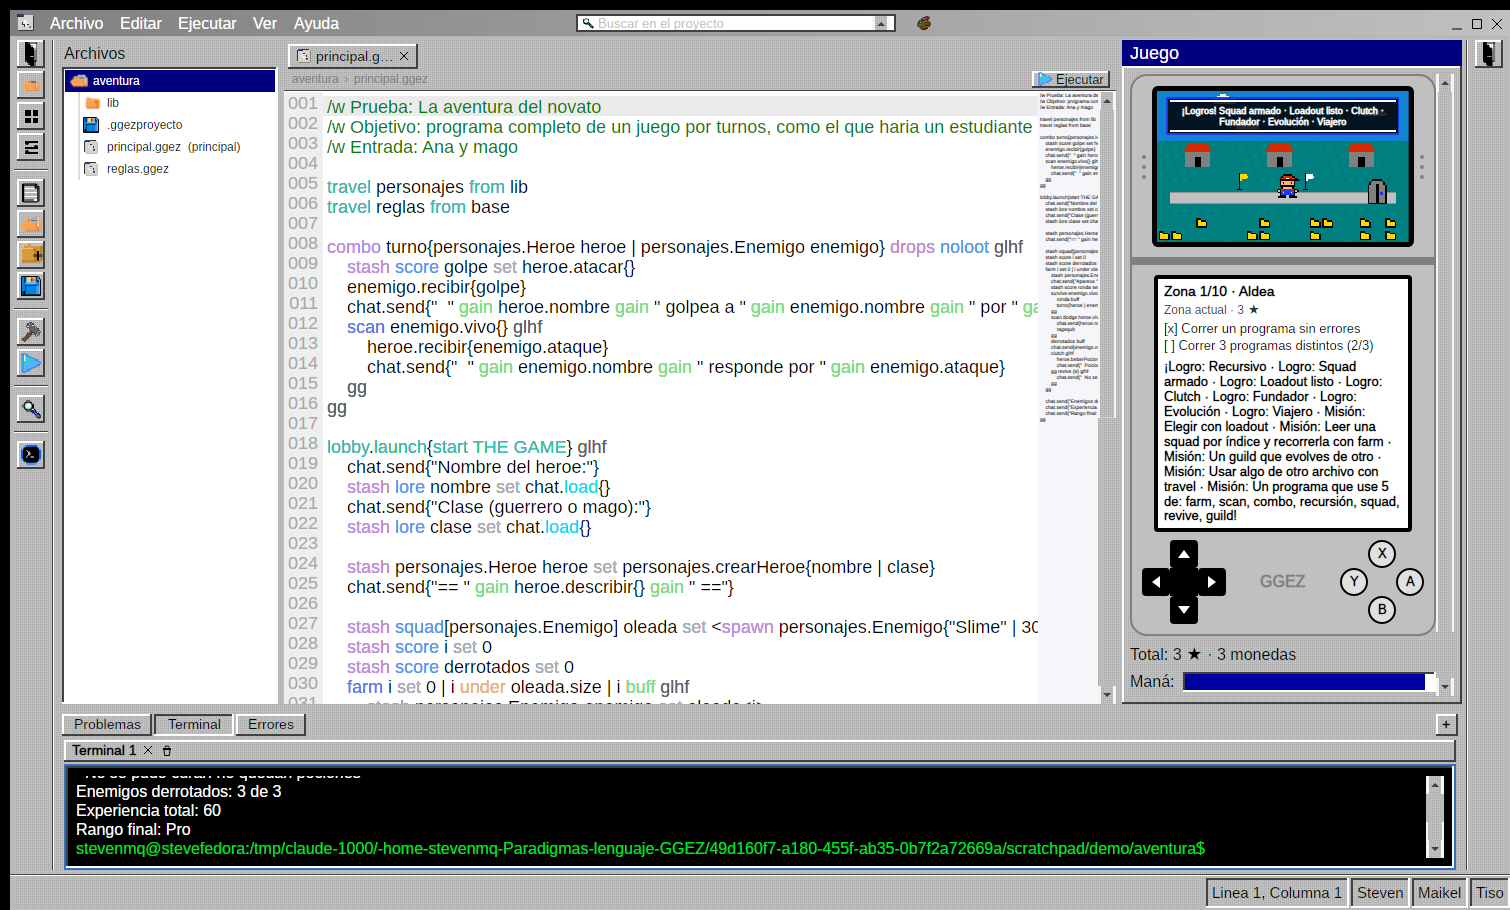
\includegraphics[width=\textwidth]{img/ide_ejecucion.png}
\caption{Ventana principal del IDE.}
\end{figure}

\begin{itemize}
  \item \textbf{Barra de menú} (arriba): Archivo, Editar, Ejecutar, Ver y Ayuda.
  \item \textbf{Barra lateral} (izquierda): íconos para cambiar entre el explorador de archivos, las extensiones y los ajustes.
  \item \textbf{Explorador}: el árbol de archivos del proyecto abierto.
  \item \textbf{Editor} (centro): pestañas con los archivos abiertos, números de línea, coloreado de sintaxis y minimapa a la derecha. Sobre el editor están la ruta del archivo y los botones de compilar (martillo) y ejecutar (reproducir).
  \item \textbf{Segmento de salida} (abajo): pestañas Terminal, Errores y Problemas.
  \item \textbf{Panel de juego} (derecha): maná, mapa del mundo, nivel actual, monedas, pistas y logros.
  \item \textbf{Barra de estado} (abajo del todo): línea y columna del cursor y otros datos.
\end{itemize}

El tamaño del explorador, del panel de juego y de la terminal se cambia arrastrando el divisor que los separa del editor; el divisor se resalta al pasar el mouse.

\manualseccion{Crear y abrir un proyecto}

\begin{enumerate}
  \item Menú \textbf{Archivo → Abrir carpeta} (\kw{Ctrl+O}) y elegir o crear una carpeta.
  \item En el explorador, clic derecho para crear archivos (\kw{.ggez}) y carpetas, renombrar o eliminar. Los archivos y carpetas que se crean, borran o editan fuera del IDE aparecen solos en el árbol, y una pestaña abierta sin cambios sin guardar se recarga con el contenido nuevo.
  \item Opcional: clic derecho sobre un archivo con \kw{lobby.launch} → \textbf{Marcar como principal}. El archivo aparece con la etiqueta «(principal)» y se usa cuando la pestaña enfocada no es un \kw{.ggez}.
\end{enumerate}

Sin proyecto abierto, también se puede crear un archivo suelto con \kw{Ctrl+N}, guardarlo y ejecutarlo.

\manualseccion{Escribir código}

\begin{itemize}
  \item El editor colorea palabras reservadas, tipos, operadores, textos y comentarios.
  \item \textbf{Autocompletado}: aparece al escribir o con \kw{Ctrl+Espacio}. Sugiere palabras reservadas, plantillas completas (por ejemplo, un \kw{farm} con sus tres partes) con su descripción, los nombres declarados en el archivo y, después de un punto, los miembros disponibles (\kw{chat.send}, \kw{lista.recruit}, lo de un módulo importado). Con las flechas se elige y con \kw{Enter} o \kw{Tab} se inserta; \kw{Esc} cierra la lista.
  \item \textbf{Minimapa}: muestra todo el archivo en miniatura a la derecha del editor; un clic salta a esa parte.
  \item Con la extensión de colores de bloques, al presionar \kw{Enter} después de \kw{glhf} el editor cierra el bloque con \kw{gg}.
  \item \kw{Ctrl+F} busca, \kw{Ctrl+H} reemplaza y \kw{Ctrl+G} va a una línea.
\end{itemize}

\begin{figure}[H]
\centering
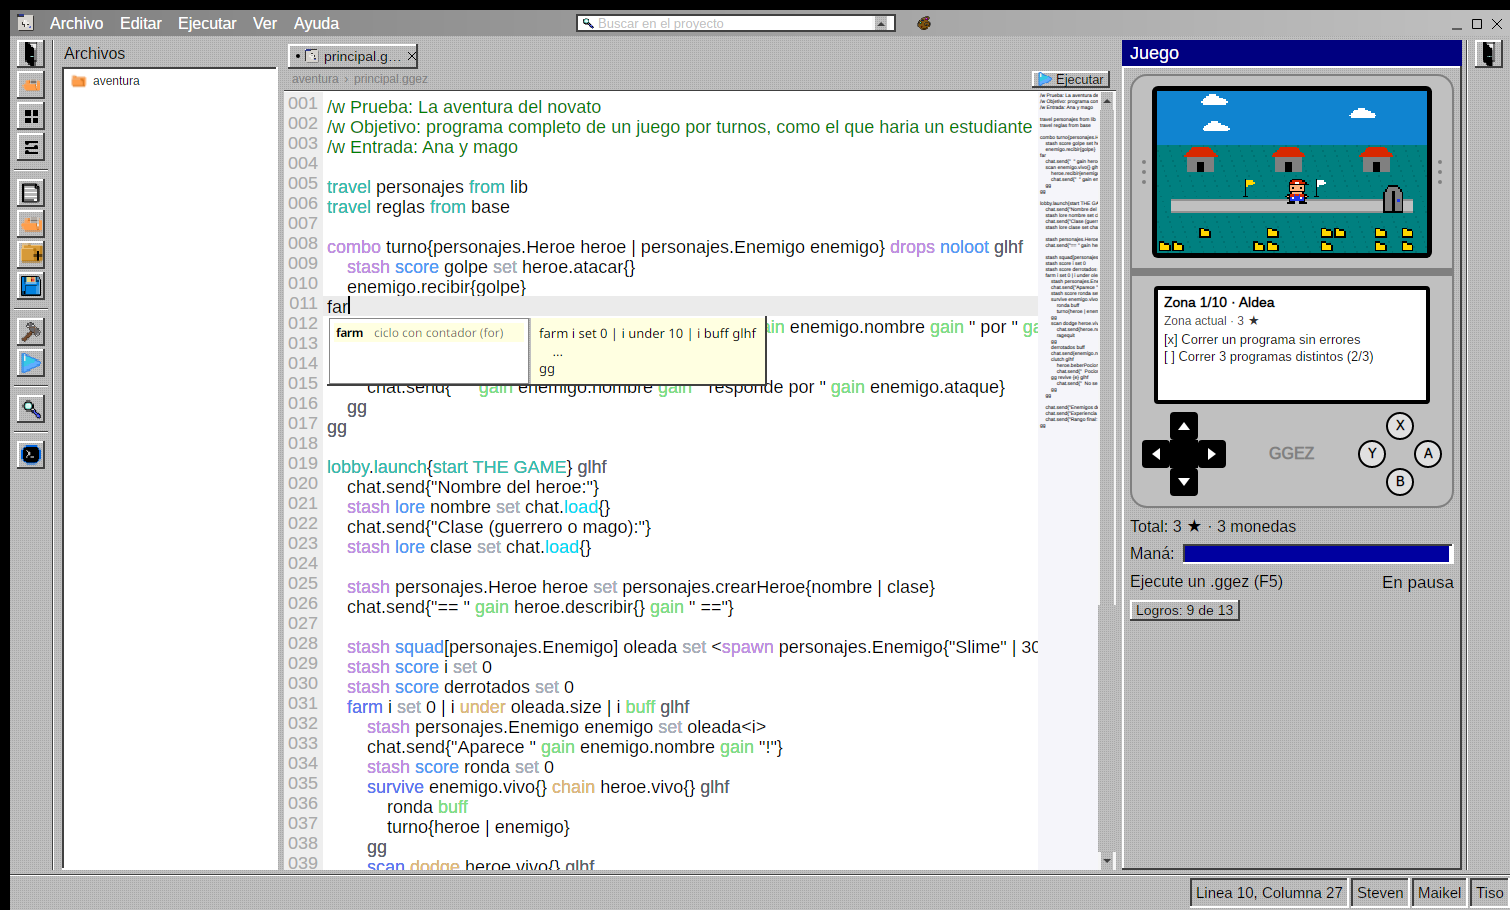
\includegraphics[width=0.92\textwidth]{img/autocompletado.png}
\caption{Autocompletado con plantillas y su descripción.}
\end{figure}

\manualseccion{Compilar y ejecutar}

\begin{itemize}
  \item \textbf{Compilar} (\kw{F6} o el martillo): revisa el archivo \kw{.ggez} de la pestaña enfocada sin ejecutarlo. Si todo está bien, la terminal muestra «Compilacion exitosa».
  \item \textbf{Ejecutar} (\kw{F5} o el botón de reproducir): compila y, si no hay errores, ejecuta el archivo \kw{.ggez} de la pestaña enfocada. Lo que imprime el programa aparece en celeste. Cuando el programa pide datos con \kw{chat.load}, se escriben en la terminal y se presiona \kw{Enter}.
  \item \kw{Ctrl+C} en la terminal detiene un programa en ejecución.
\end{itemize}

\manualseccion{Corregir errores}

\begin{enumerate}
  \item Si hay un error, la terminal lo muestra en rojo y la pestaña \textbf{Problemas} lo lista con su tipo, archivo, línea y posible causa.
  \item Un clic sobre el problema abre el archivo y lleva el cursor a la línea.
  \item Las advertencias aparecen en amarillo y no impiden ejecutar.
  \item Menú \textbf{Ejecutar → Ver errores} abre la pestaña de errores.
\end{enumerate}

\manualseccion{Terminal}

La terminal permite escribir comandos del sistema y tiene comandos propios: \kw{cd}, \kw{clear}, \kw{exit} y \kw{help}. Con el botón \textbf{+} se abren hasta cuatro terminales, una al lado de la otra. La primera terminal es siempre la terminal de \ggez, donde se compila y ejecuta. Con la extensión de Claude instalada, al escribir \kw{claude} en ella se abre otra terminal al lado con el asistente; en sus menús se elige con las flechas y \kw{Enter}.

Colores de la terminal: verde el indicador, blanco lo que escribe el usuario, celeste la salida del programa, rojo los errores y amarillo los avisos y advertencias.

\manualseccion{Modo de juego}

\begin{itemize}
  \item \textbf{Maná}: la barra muestra cuánto gastó el último programa.
  \item \textbf{Mapa}: muestra la zona actual y sus misiones; las flechas recorren las zonas. Al cumplir todas las misiones de una zona se abre la siguiente.
  \item \textbf{Niveles}: abrir la carpeta de un nivel (con \kw{nivel.json}) y ejecutar el archivo; el panel muestra cuántas pruebas pasaron y las estrellas ganadas.
  \item \textbf{Pistas}: el botón de pista gasta una moneda y muestra la siguiente pista del nivel.
  \item \textbf{Logros}: la lista muestra los obtenidos y los pendientes.
\end{itemize}

\manualseccion{Extensiones y ajustes}

En la vista de \textbf{Extensiones} se instalan y desinstalan complementos con un clic, entre ellos los temas desbloqueados con estrellas. En \textbf{Ajustes} se cambian el tamaño de letra, el zoom y otras preferencias del editor. Todo se conserva al cerrar el IDE, junto con las pestañas abiertas.

\begin{figure}[H]
\centering
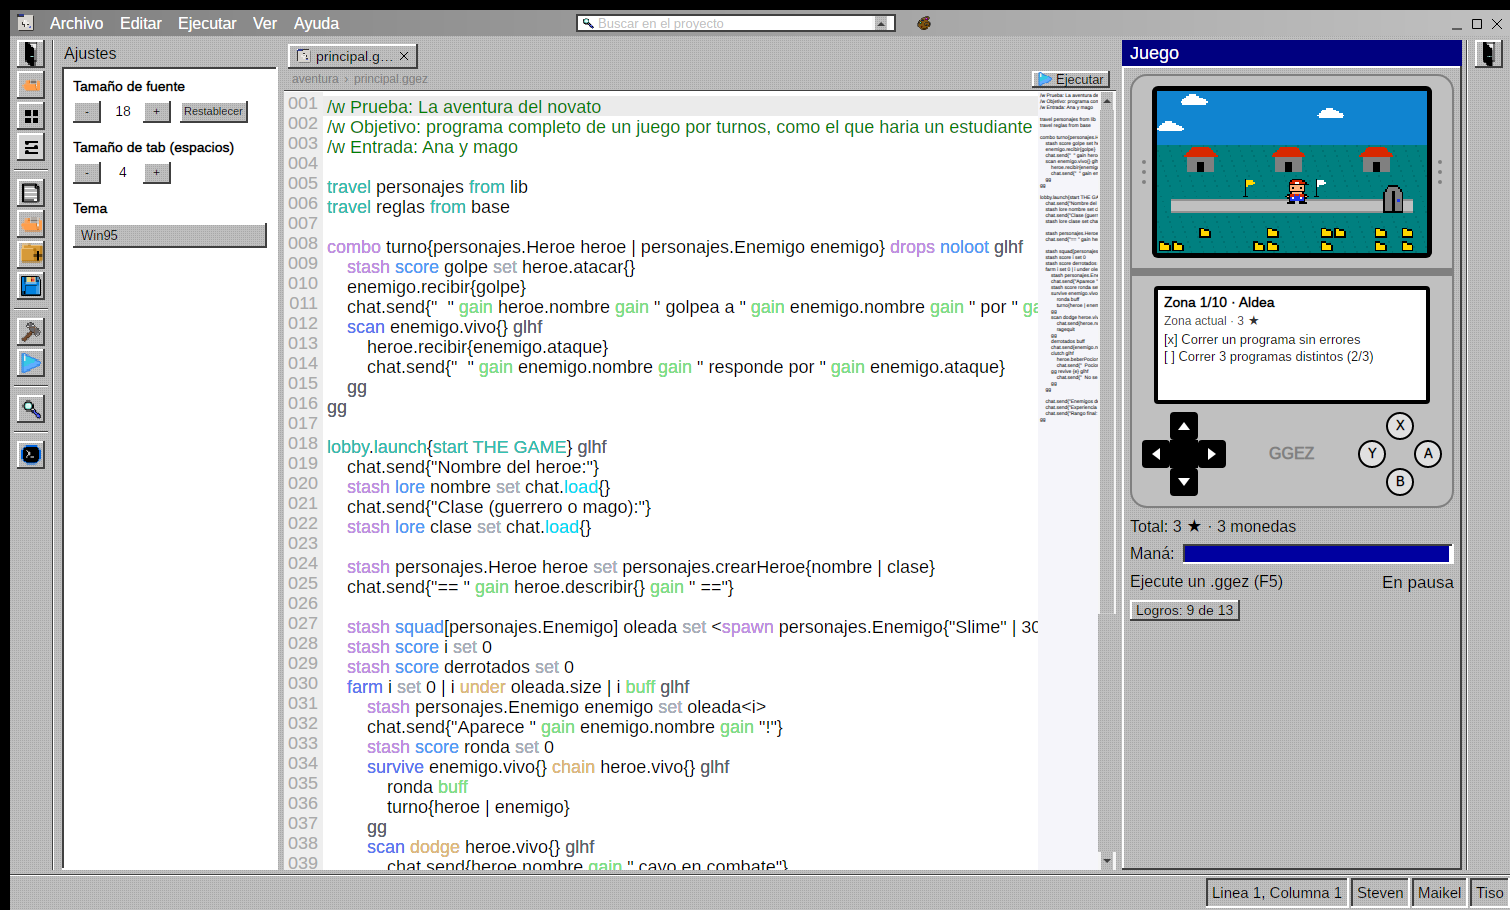
\includegraphics[width=0.92\textwidth]{img/ajustes.png}
\caption{Vista de ajustes.}
\end{figure}

\manualseccion{Ayuda}

\begin{itemize}
  \item \textbf{Ayuda → Sintaxis de GGEZ}: referencia completa del lenguaje, con cada ejemplo junto a su equivalente en Java.
  \item \textbf{Ayuda → Atajos de teclado} (\kw{F1}): lista de todos los atajos.
  \item \textbf{Ayuda → Acerca de}: versión e integrantes.
\end{itemize}

\begin{figure}[H]
\centering
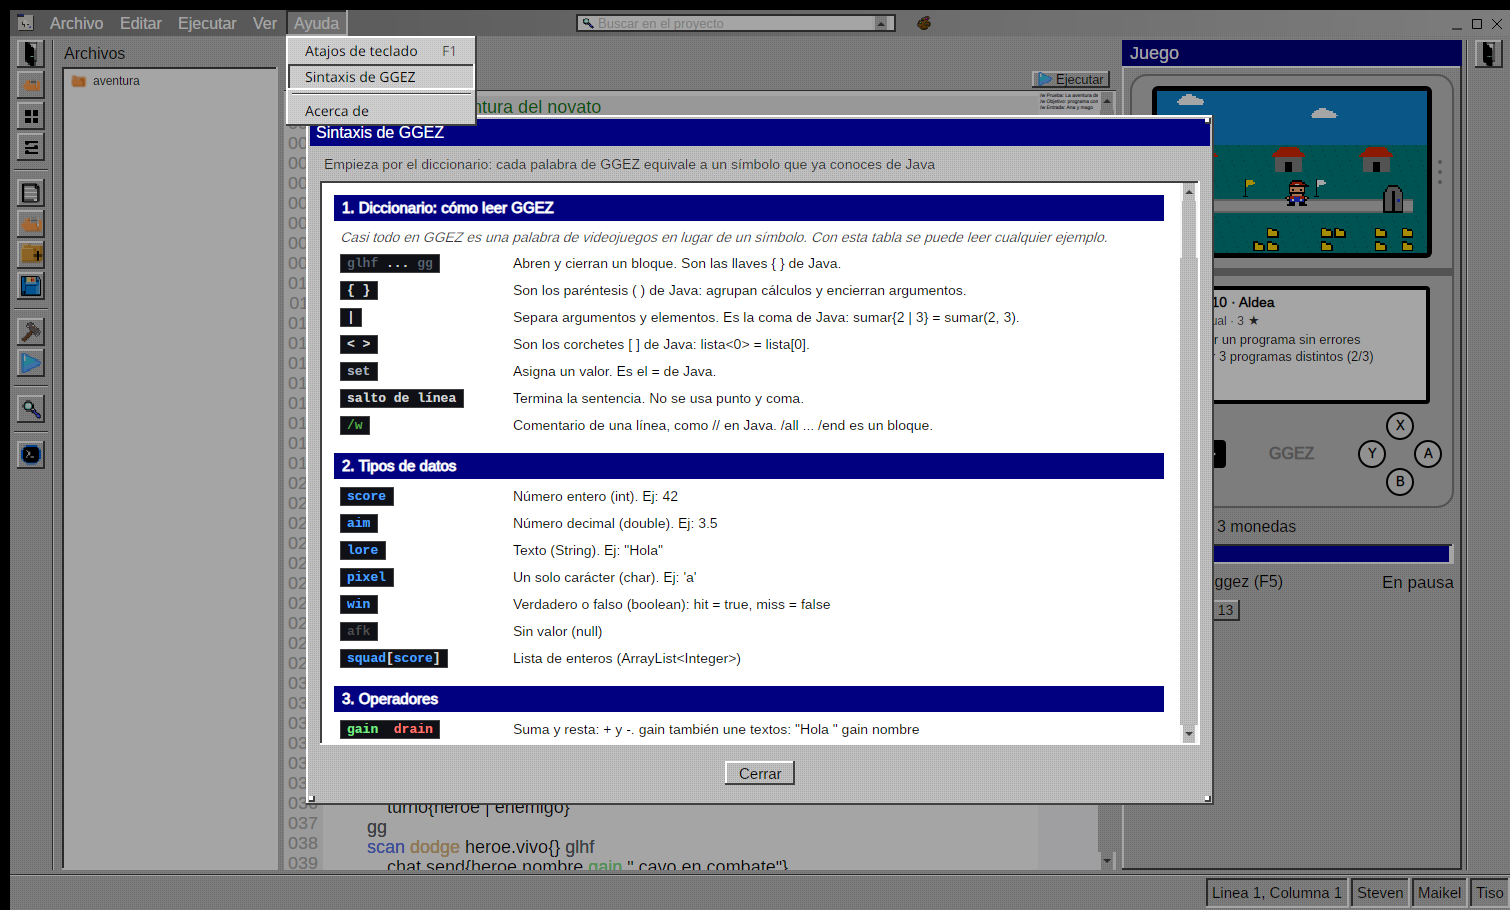
\includegraphics[width=0.92\textwidth]{img/sintaxis.png}
\caption{Referencia del lenguaje con el equivalente en Java.}
\end{figure}

\begin{figure}[H]
\centering
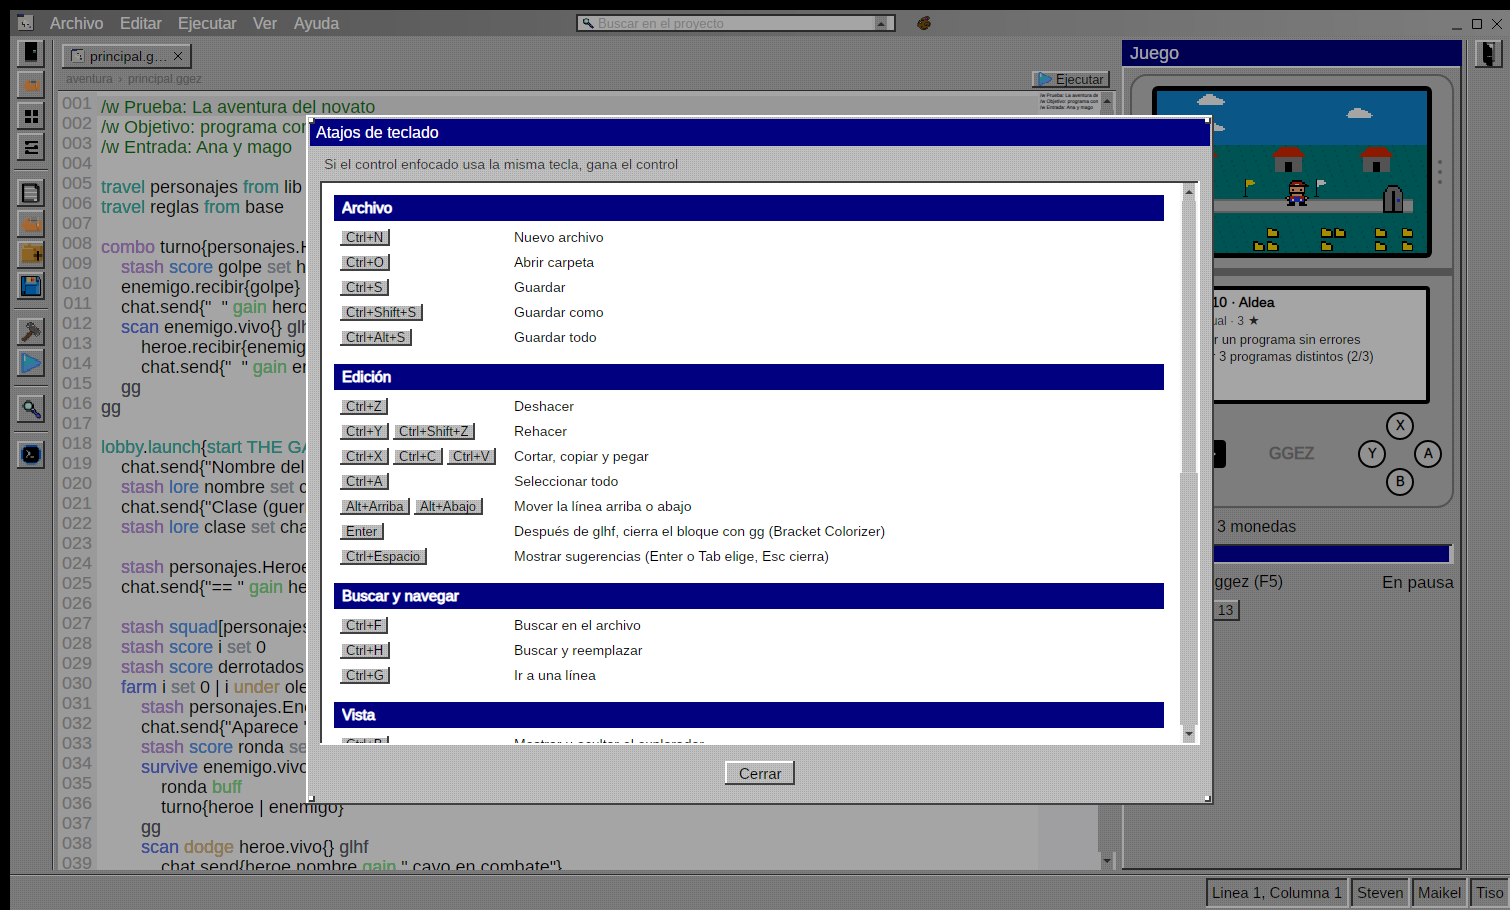
\includegraphics[width=0.92\textwidth]{img/atajos.png}
\caption{Atajos de teclado.}
\end{figure}

\manualseccion{Atajos principales}

\begin{longtable}{|p{5cm}|p{9.4cm}|}\hline
\cab\textbf{Atajo} & \textbf{Acción} \\\hline\endhead
\kw{F5} / \kw{F6} & Ejecutar / Compilar \\\hline
\kw{F1} & Mostrar los atajos \\\hline
\kw{Ctrl+N}, \kw{Ctrl+O} & Nuevo archivo, abrir carpeta \\\hline
\kw{Ctrl+S}, \kw{Ctrl+Alt+S} & Guardar, guardar todo \\\hline
\kw{Ctrl+Z}, \kw{Ctrl+Y} & Deshacer, rehacer \\\hline
\kw{Alt+Arriba} / \kw{Alt+Abajo} & Mover la línea \\\hline
\kw{Ctrl+Espacio} & Sugerencias de autocompletado \\\hline
\kw{Ctrl+F}, \kw{Ctrl+H}, \kw{Ctrl+G} & Buscar, reemplazar, ir a línea \\\hline
\kw{Ctrl+B}, \kw{Ctrl+J} & Mostrar u ocultar explorador y terminal \\\hline
\kw{Ctrl++}, \kw{Ctrl+-}, \kw{Ctrl+0} & Zoom \\\hline
\kw{Ctrl+C} (en la terminal) & Interrumpir el programa \\\hline
\end{longtable}

